% Created by tikzDevice version 0.8.1 on 2015-11-21 10:22:04
% !TEX encoding = UTF-8 Unicode
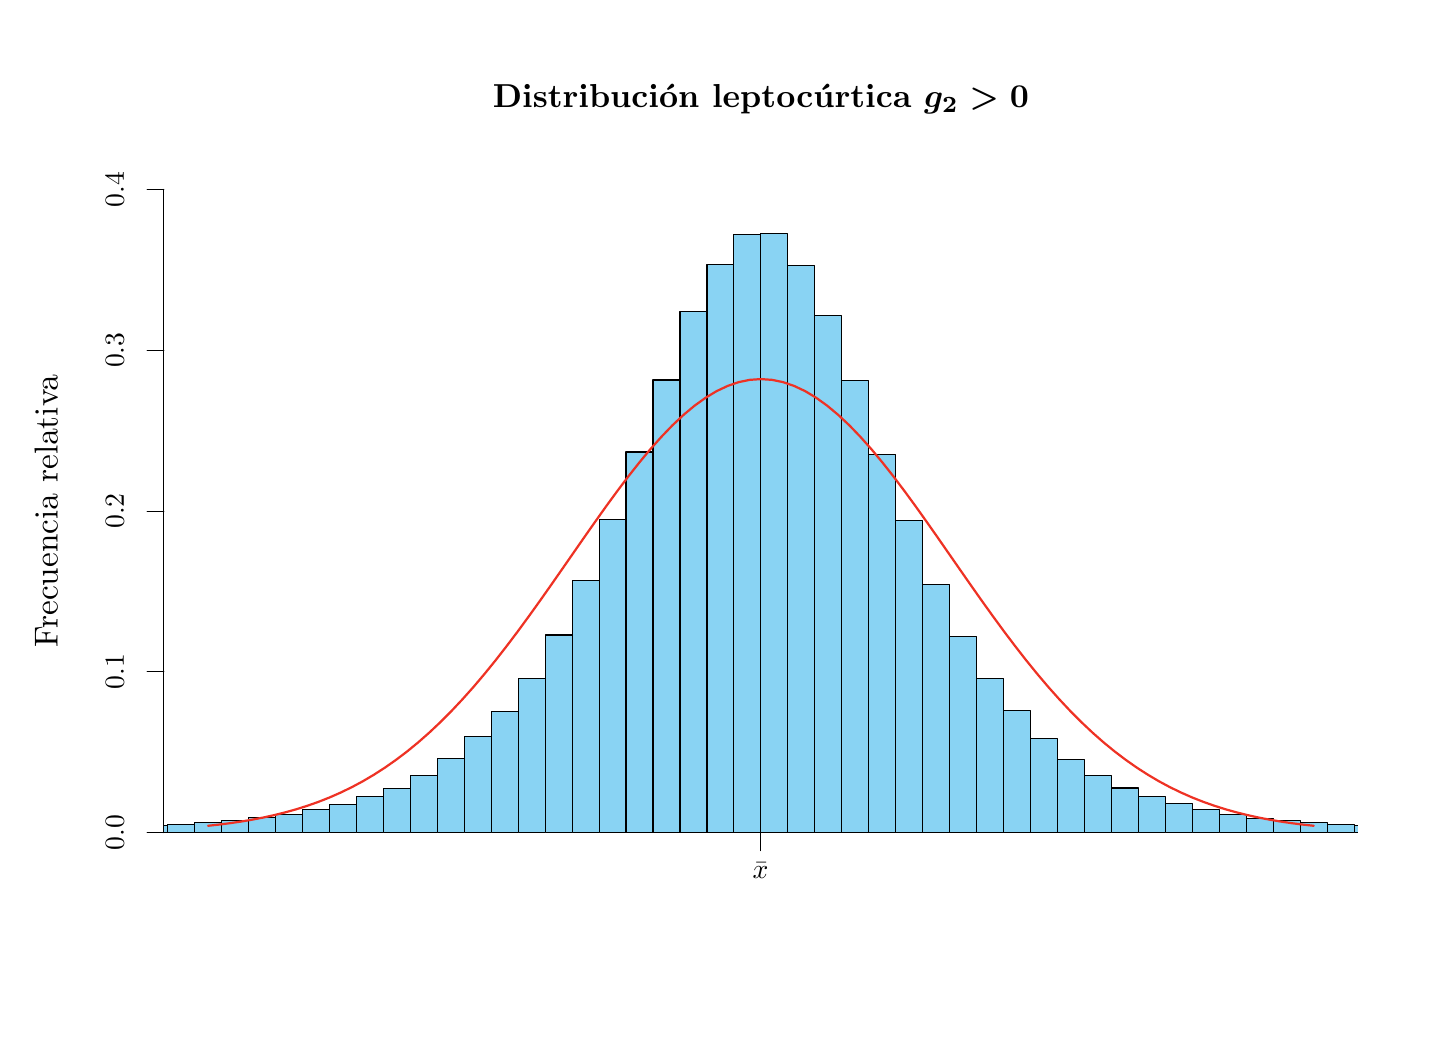
\begin{tikzpicture}[x=1pt,y=1pt]
\definecolor{fillColor}{RGB}{255,255,255}
\path[use as bounding box,fill=fillColor,fill opacity=0.00] (0,0) rectangle (505.89,361.35);
\begin{scope}
\path[clip] (  0.00,  0.00) rectangle (505.89,361.35);
\definecolor{drawColor}{RGB}{0,0,0}

\node[text=drawColor,anchor=base,inner sep=0pt, outer sep=0pt, scale=  1.20, font=\boldmath] at (264.94,332.61)
{\bfseries Distribución leptocúrtica $g_2>0$};

\node[text=drawColor,rotate= 90.00,anchor=base,inner sep=0pt, outer sep=0pt, scale=  1.20] at ( 10.80,186.67)
{Frecuencia relativa};
\end{scope}
\begin{scope}
\path[clip] ( 49.20, 61.20) rectangle (480.69,312.15);
\definecolor{drawColor}{RGB}{0,0,0}
\definecolor{fillColor}{RGB}{137,211,243}

\path[draw=drawColor,line width= 0.4pt,line join=round,line cap=round,fill=fillColor] ( -7.90, 70.49) rectangle (  1.84, 71.43);

\path[draw=drawColor,line width= 0.4pt,line join=round,line cap=round,fill=fillColor] (  1.84, 70.49) rectangle ( 11.59, 71.73);

\path[draw=drawColor,line width= 0.4pt,line join=round,line cap=round,fill=fillColor] ( 11.59, 70.49) rectangle ( 21.33, 71.97);

\path[draw=drawColor,line width= 0.4pt,line join=round,line cap=round,fill=fillColor] ( 21.33, 70.49) rectangle ( 31.08, 72.32);

\path[draw=drawColor,line width= 0.4pt,line join=round,line cap=round,fill=fillColor] ( 31.08, 70.49) rectangle ( 40.82, 72.61);

\path[draw=drawColor,line width= 0.4pt,line join=round,line cap=round,fill=fillColor] ( 40.82, 70.49) rectangle ( 50.56, 72.95);

\path[draw=drawColor,line width= 0.4pt,line join=round,line cap=round,fill=fillColor] ( 50.56, 70.49) rectangle ( 60.31, 73.34);

\path[draw=drawColor,line width= 0.4pt,line join=round,line cap=round,fill=fillColor] ( 60.31, 70.49) rectangle ( 70.05, 74.05);

\path[draw=drawColor,line width= 0.4pt,line join=round,line cap=round,fill=fillColor] ( 70.05, 70.49) rectangle ( 79.80, 74.81);

\path[draw=drawColor,line width= 0.4pt,line join=round,line cap=round,fill=fillColor] ( 79.80, 70.49) rectangle ( 89.54, 75.86);

\path[draw=drawColor,line width= 0.4pt,line join=round,line cap=round,fill=fillColor] ( 89.54, 70.49) rectangle ( 99.29, 77.18);

\path[draw=drawColor,line width= 0.4pt,line join=round,line cap=round,fill=fillColor] ( 99.29, 70.49) rectangle (109.03, 78.74);

\path[draw=drawColor,line width= 0.4pt,line join=round,line cap=round,fill=fillColor] (109.03, 70.49) rectangle (118.78, 80.76);

\path[draw=drawColor,line width= 0.4pt,line join=round,line cap=round,fill=fillColor] (118.78, 70.49) rectangle (128.52, 83.39);

\path[draw=drawColor,line width= 0.4pt,line join=round,line cap=round,fill=fillColor] (128.52, 70.49) rectangle (138.27, 86.54);

\path[draw=drawColor,line width= 0.4pt,line join=round,line cap=round,fill=fillColor] (138.27, 70.49) rectangle (148.01, 91.02);

\path[draw=drawColor,line width= 0.4pt,line join=round,line cap=round,fill=fillColor] (148.01, 70.49) rectangle (157.75, 97.14);

\path[draw=drawColor,line width= 0.4pt,line join=round,line cap=round,fill=fillColor] (157.75, 70.49) rectangle (167.50,105.09);

\path[draw=drawColor,line width= 0.4pt,line join=round,line cap=round,fill=fillColor] (167.50, 70.49) rectangle (177.24,114.25);

\path[draw=drawColor,line width= 0.4pt,line join=round,line cap=round,fill=fillColor] (177.24, 70.49) rectangle (186.99,126.25);

\path[draw=drawColor,line width= 0.4pt,line join=round,line cap=round,fill=fillColor] (186.99, 70.49) rectangle (196.73,141.90);

\path[draw=drawColor,line width= 0.4pt,line join=round,line cap=round,fill=fillColor] (196.73, 70.49) rectangle (206.48,161.66);

\path[draw=drawColor,line width= 0.4pt,line join=round,line cap=round,fill=fillColor] (206.48, 70.49) rectangle (216.22,183.76);

\path[draw=drawColor,line width= 0.4pt,line join=round,line cap=round,fill=fillColor] (216.22, 70.49) rectangle (225.97,208.02);

\path[draw=drawColor,line width= 0.4pt,line join=round,line cap=round,fill=fillColor] (225.97, 70.49) rectangle (235.71,234.04);

\path[draw=drawColor,line width= 0.4pt,line join=round,line cap=round,fill=fillColor] (235.71, 70.49) rectangle (245.46,258.92);

\path[draw=drawColor,line width= 0.4pt,line join=round,line cap=round,fill=fillColor] (245.46, 70.49) rectangle (255.20,275.69);

\path[draw=drawColor,line width= 0.4pt,line join=round,line cap=round,fill=fillColor] (255.20, 70.49) rectangle (264.94,286.56);

\path[draw=drawColor,line width= 0.4pt,line join=round,line cap=round,fill=fillColor] (264.94, 70.49) rectangle (274.69,286.83);

\path[draw=drawColor,line width= 0.4pt,line join=round,line cap=round,fill=fillColor] (274.69, 70.49) rectangle (284.43,275.51);

\path[draw=drawColor,line width= 0.4pt,line join=round,line cap=round,fill=fillColor] (284.43, 70.49) rectangle (294.18,257.22);

\path[draw=drawColor,line width= 0.4pt,line join=round,line cap=round,fill=fillColor] (294.18, 70.49) rectangle (303.92,233.82);

\path[draw=drawColor,line width= 0.4pt,line join=round,line cap=round,fill=fillColor] (303.92, 70.49) rectangle (313.67,207.22);

\path[draw=drawColor,line width= 0.4pt,line join=round,line cap=round,fill=fillColor] (313.67, 70.49) rectangle (323.41,183.13);

\path[draw=drawColor,line width= 0.4pt,line join=round,line cap=round,fill=fillColor] (323.41, 70.49) rectangle (333.16,160.21);

\path[draw=drawColor,line width= 0.4pt,line join=round,line cap=round,fill=fillColor] (333.16, 70.49) rectangle (342.90,141.38);

\path[draw=drawColor,line width= 0.4pt,line join=round,line cap=round,fill=fillColor] (342.90, 70.49) rectangle (352.65,126.27);

\path[draw=drawColor,line width= 0.4pt,line join=round,line cap=round,fill=fillColor] (352.65, 70.49) rectangle (362.39,114.52);

\path[draw=drawColor,line width= 0.4pt,line join=round,line cap=round,fill=fillColor] (362.39, 70.49) rectangle (372.14,104.42);

\path[draw=drawColor,line width= 0.4pt,line join=round,line cap=round,fill=fillColor] (372.14, 70.49) rectangle (381.88, 96.87);

\path[draw=drawColor,line width= 0.4pt,line join=round,line cap=round,fill=fillColor] (381.88, 70.49) rectangle (391.62, 90.97);

\path[draw=drawColor,line width= 0.4pt,line join=round,line cap=round,fill=fillColor] (391.62, 70.49) rectangle (401.37, 86.61);

\path[draw=drawColor,line width= 0.4pt,line join=round,line cap=round,fill=fillColor] (401.37, 70.49) rectangle (411.11, 83.56);

\path[draw=drawColor,line width= 0.4pt,line join=round,line cap=round,fill=fillColor] (411.11, 70.49) rectangle (420.86, 80.92);

\path[draw=drawColor,line width= 0.4pt,line join=round,line cap=round,fill=fillColor] (420.86, 70.49) rectangle (430.60, 78.90);

\path[draw=drawColor,line width= 0.4pt,line join=round,line cap=round,fill=fillColor] (430.60, 70.49) rectangle (440.35, 77.13);

\path[draw=drawColor,line width= 0.4pt,line join=round,line cap=round,fill=fillColor] (440.35, 70.49) rectangle (450.09, 75.58);

\path[draw=drawColor,line width= 0.4pt,line join=round,line cap=round,fill=fillColor] (450.09, 70.49) rectangle (459.84, 74.90);

\path[draw=drawColor,line width= 0.4pt,line join=round,line cap=round,fill=fillColor] (459.84, 70.49) rectangle (469.58, 73.98);

\path[draw=drawColor,line width= 0.4pt,line join=round,line cap=round,fill=fillColor] (469.58, 70.49) rectangle (479.33, 73.42);

\path[draw=drawColor,line width= 0.4pt,line join=round,line cap=round,fill=fillColor] (479.33, 70.49) rectangle (489.07, 72.92);

\path[draw=drawColor,line width= 0.4pt,line join=round,line cap=round,fill=fillColor] (489.07, 70.49) rectangle (498.81, 72.51);

\path[draw=drawColor,line width= 0.4pt,line join=round,line cap=round,fill=fillColor] (498.81, 70.49) rectangle (508.56, 72.10);
\end{scope}
\begin{scope}
\path[clip] (  0.00,  0.00) rectangle (505.89,361.35);
\definecolor{drawColor}{RGB}{0,0,0}

\path[draw=drawColor,line width= 0.4pt,line join=round,line cap=round] (264.79, 70.49) -- (264.79, 64);

\node[text=drawColor,anchor=base,inner sep=0pt, outer sep=0pt, scale=  1.00] at (264.79, 54) {$\bar x$};

\path[draw=drawColor,line width= 0.4pt,line join=round,line cap=round] ( 49.20, 70.49) -- ( 49.20,302.86);

\path[draw=drawColor,line width= 0.4pt,line join=round,line cap=round] ( 49.20, 70.49) -- ( 43.20, 70.49);

\path[draw=drawColor,line width= 0.4pt,line join=round,line cap=round] ( 49.20,128.58) -- ( 43.20,128.58);

\path[draw=drawColor,line width= 0.4pt,line join=round,line cap=round] ( 49.20,186.67) -- ( 43.20,186.67);

\path[draw=drawColor,line width= 0.4pt,line join=round,line cap=round] ( 49.20,244.77) -- ( 43.20,244.77);

\path[draw=drawColor,line width= 0.4pt,line join=round,line cap=round] ( 49.20,302.86) -- ( 43.20,302.86);

\node[text=drawColor,rotate= 90.00,anchor=base,inner sep=0pt, outer sep=0pt, scale=  1.00] at ( 34.80, 70.49) {0.0};

\node[text=drawColor,rotate= 90.00,anchor=base,inner sep=0pt, outer sep=0pt, scale=  1.00] at ( 34.80,128.58) {0.1};

\node[text=drawColor,rotate= 90.00,anchor=base,inner sep=0pt, outer sep=0pt, scale=  1.00] at ( 34.80,186.67) {0.2};

\node[text=drawColor,rotate= 90.00,anchor=base,inner sep=0pt, outer sep=0pt, scale=  1.00] at ( 34.80,244.77) {0.3};

\node[text=drawColor,rotate= 90.00,anchor=base,inner sep=0pt, outer sep=0pt, scale=  1.00] at ( 34.80,302.86) {0.4};
\end{scope}
\begin{scope}
\path[clip] ( 49.20, 61.20) rectangle (480.69,312.15);
\definecolor{drawColor}{RGB}{238,50,36}

\path[draw=drawColor,line width= 0.8pt,line join=round,line cap=round] ( 65.18, 72.95) --
	( 69.18, 73.39) --
	( 73.17, 73.90) --
	( 77.17, 74.49) --
	( 81.16, 75.17) --
	( 85.16, 75.94) --
	( 89.15, 76.82) --
	( 93.15, 77.82) --
	( 97.14, 78.94) --
	(101.14, 80.21) --
	(105.13, 81.62) --
	(109.13, 83.20) --
	(113.12, 84.96) --
	(117.12, 86.90) --
	(121.11, 89.04) --
	(125.11, 91.40) --
	(129.11, 93.97) --
	(133.10, 96.77) --
	(137.10, 99.80) --
	(141.09,103.07) --
	(145.09,106.59) --
	(149.08,110.35) --
	(153.08,114.36) --
	(157.07,118.61) --
	(161.07,123.09) --
	(165.06,127.80) --
	(169.06,132.72) --
	(173.05,137.84) --
	(177.05,143.13) --
	(181.04,148.58) --
	(185.04,154.15) --
	(189.03,159.81) --
	(193.03,165.55) --
	(197.03,171.31) --
	(201.02,177.06) --
	(205.02,182.76) --
	(209.01,188.37) --
	(213.01,193.84) --
	(217.00,199.13) --
	(221.00,204.20) --
	(224.99,209.01) --
	(228.99,213.50) --
	(232.98,217.65) --
	(236.98,221.41) --
	(240.97,224.74) --
	(244.97,227.62) --
	(248.96,230.02) --
	(252.96,231.90) --
	(256.95,233.27) --
	(260.95,234.09) --
	(264.94,234.36) --
	(268.94,234.09) --
	(272.94,233.27) --
	(276.93,231.90) --
	(280.93,230.02) --
	(284.92,227.62) --
	(288.92,224.74) --
	(292.91,221.41) --
	(296.91,217.65) --
	(300.90,213.50) --
	(304.90,209.01) --
	(308.89,204.20) --
	(312.89,199.13) --
	(316.88,193.84) --
	(320.88,188.37) --
	(324.87,182.76) --
	(328.87,177.06) --
	(332.86,171.31) --
	(336.86,165.55) --
	(340.86,159.81) --
	(344.85,154.15) --
	(348.85,148.58) --
	(352.84,143.13) --
	(356.84,137.84) --
	(360.83,132.72) --
	(364.83,127.80) --
	(368.82,123.09) --
	(372.82,118.61) --
	(376.81,114.36) --
	(380.81,110.35) --
	(384.80,106.59) --
	(388.80,103.07) --
	(392.79, 99.80) --
	(396.79, 96.77) --
	(400.78, 93.97) --
	(404.78, 91.40) --
	(408.77, 89.04) --
	(412.77, 86.90) --
	(416.77, 84.96) --
	(420.76, 83.20) --
	(424.76, 81.62) --
	(428.75, 80.21) --
	(432.75, 78.94) --
	(436.74, 77.82) --
	(440.74, 76.82) --
	(444.73, 75.94) --
	(448.73, 75.17) --
	(452.72, 74.49) --
	(456.72, 73.90) --
	(460.71, 73.39) --
	(464.71, 72.95);
\end{scope}
\end{tikzpicture}
